\documentclass[a4paper, 12pt, italian]{report}
\usepackage[a4paper, top=3cm, bottom=3cm, left=3cm, right=3cm, headheight=15pt]{geometry}
\usepackage[italian,provide=*]{babel}
%\usepackage[latin1]{inputenc}
%\usepackage[T1]{fontenc}
\usepackage{graphicx}
\usepackage{float}
\usepackage[centertags]{amsmath}
\usepackage{amsfonts}
\usepackage{amssymb}
\usepackage{amsthm}
\usepackage{amsmath}
\usepackage{newlfont}
\usepackage{fancyhdr}
\usepackage{tesisty}
\usepackage{titlesec}
\usepackage{tocloft}
\usepackage[T1]{fontenc}
\usepackage{fancyvrb}
\usepackage{listings}

\usepackage{algorithm}
\usepackage{algorithmicx}
\usepackage[noend]{algpseudocode}

\makeatletter
\def\BState{\State\hskip-\ALG@thistlm}
\makeatother
\algdef{SE}[DOWHILE]{Do}{doWhile}{\algorithmicdo}[1]{\algorithmicwhile\ #1}%

\algdef{SE}[VARIABLES]{Variables}{EndVariables}
   {\algorithmicvariables}
   {\algorithmicend\ \algorithmicvariables}
\algnewcommand{\algorithmicvariables}{\textbf{global variables}}

\addto\captionsitalian{%
\renewcommand{\lstlistingname}{Codice}}
\addto\captionsitalian{%
\renewcommand{\lstlistlistingname}{Elenco dei codici}}
\floatname{algorithm}{Algoritmo}
\addto\captionsitalian{%
\renewcommand{\listalgorithmname}{Elenco degli algoritmi}}
\newcommand{\myalgosize}{\scriptsize}

%necessario per commenti
\usepackage[table]{xcolor}
\usepackage{xcolor}

%-------------------------------
% DEFINIZIONE DEGLI ENVIRONMENT
%-------------------------------

\newtheorem{obs}{Osservazione}[section]
\newenvironment{oss}
    {\begin{obs}\begin{normalfont}}
    {\hfill $\square \!\!\!\!\checkmark$ \end{normalfont}\end{obs}}

\newtheorem{pro}{Problema}[chapter]
\newenvironment{prob}
    {\begin{pro}\begin{normalfont}}
    {\hfill $\spadesuit$ \end{normalfont}\end{pro}}

\newtheorem{teor}{Teorema}[section]
\newenvironment{teorema}
    {\begin{teor}\textit }
    {\hfill  \end{teor}}

\newtheorem{defn}{Definizione}[section]
\newenvironment{de}
    {\begin{defn}\begin{normalfont}}
    {\hfill $\clubsuit$ \end{normalfont}\end{defn}}

%-----------------------------
% CONFIGURAZIONE DELLA PAGINA
%-----------------------------

\hfuzz2pt % Don't bother to report over-full boxes if over-edge is < 2pt

\fancypagestyle{plain}{
\fancyhead{}\renewcommand{\headrulewidth}{0pt} } \pagestyle{fancy}
\renewcommand{\chaptermark}[1]{\markboth{\small CAP. \thechapter \textit{ #1}} {} }
\renewcommand{\sectionmark}[1]{\markright{\small  \thesection \textit{ #1}} {} }
\fancyhead{}
\fancyfoot{}
\fancyhead[R]{\rightmark} \fancyfoot[L]{\leftmark}
\fancyfoot[R]{\thepage}
\renewcommand{\headrulewidth}{0.3pt}
\renewcommand{\footrulewidth}{0.3pt}

\numberwithin{equation}{section}
\renewcommand{\theequation}{\thesection.\arabic{equation}}

\setcounter{secnumdepth}{3} % Abilita la numerazione fino alle sottosottosezioni
\setcounter{tocdepth}{3} % Abilita l'inclusione delle sottosottosezioni nell'indice


 

% Support for pandoc-generated LaTeX & listings styling
\usepackage[plainpages=false,pdfpagelabels]{hyperref}
\usepackage{booktabs}
\usepackage{longtable}
\usepackage{calc}
\usepackage{textcomp}
\setlength{\headheight}{15pt}
\providecommand{\tightlist}{%
  \setlength{\itemsep}{0pt}\setlength{\parskip}{0pt}}
\newcommand{\passthrough}[1]{#1}

% Search images in parent root as well
\graphicspath{{../}{./}}

% Global image constraints: never exceed text width or height
\makeatletter
\def\maxwidth{\ifdim\Gin@nat@width>\linewidth\linewidth\else\Gin@nat@width\fi}
\def\maxheight{\ifdim\Gin@nat@height>\textheight\textheight\else\Gin@nat@height\fi}
\makeatother
\setkeys{Gin}{width=\maxwidth,height=\maxheight,keepaspectratio}

\lstset{
    basicstyle=\ttfamily\footnotesize,
    breaklines=true,
    numbers=left,
    numberstyle=\tiny\color{gray},
    keywordstyle=\color{blue}\bfseries,
    commentstyle=\color{olive}\itshape,
    stringstyle=\color{teal},
    showstringspaces=false,
    frame=lines
}

\begin{document}



%\dedicate{Inserire la dedica}

\titoloTesi{sbergz on the sburgz} 
\anno{2023-2024}
\relatore{Pierpaolo Loreti}
\correlatore{Ing. Francesco Mancini}
\candidato{Davide Luci}
\intestazione 
\linespread{1.15}\selectfont 
%------------------------------------------------
% INTRODUZIONE E RINGRAZIAMENTI (NON MODIFICARE)
%------------------------------------------------

\fancypagestyle{plain}{
\fancyhead{}\renewcommand{\headrulewidth}{0pt} } \pagestyle{fancy}
\renewcommand{\chaptermark}[1]{\markboth{\small Cap. \thechapter \textit{ #1}} {} }
\renewcommand{\sectionmark}[1]{\markright{\small  \S \thesection \textit{ #1}} {} }
\fancyhead{}
\fancyfoot{}
\fancyhead[R]{\rightmark} \fancyfoot[L]{\leftmark}
\fancyfoot[R]{\thepage}
\renewcommand{\headrulewidth}{0.3pt}
\renewcommand{\footrulewidth}{0.3pt}

\pagenumbering{Roman} \tableofcontents
\newpage
\pagenumbering{arabic}
\setcounter{page}{1}




\fancyhead[R]{Introduzione} \fancyfoot[L]{Introduzione}
% Capitolo: Introduzione
\chapter{Introduzione}

\section{Introduzione al Problema}\label{introduzione-al-problema}

Nel lavoro di tesi, vogliamo gestire una competizione CTF.

Di solito, in una competizione CTF, uno o piu\textquotesingle{} utenti
(eventualmente organizzati in team) si sfidano per risolvere
un\textquotesingle insieme di challenge. Generalmente una challenge vuol
dire: recuperare una \textbf{flag}.

Ci sono vari tipi di competizioni CTF, tra cui:

\begin{itemize}
\tightlist
\item
  \textbf{Jeopardy}: gli utenti devono risolvere vari problemi, la cui
  flag e\textquotesingle{} di solito una stringa del tipo
  \passthrough{\lstinline!\{hai\_trovato\_la\_flag\}!}
\item
  \textbf{Attacco e Difesa}: e\textquotesingle{} un tipo di competizione
  dove ogni team, deve recuperare una o piu flag attaccando i sistemi
  dei team avversare, mentre ognuno si occupa di difendere il proprio
  sistema.
\end{itemize}

In particolare, con il nostro lavoro, vogliamo gestire uno o
piu\textquotesingle{} sistemi vulnerabili ad un qualche tipo di attacco.

La flag si ottiene difendendo il sistema, ossia \emph{"patchando"} la
vulnerabilita. Dunque la flag non e\textquotesingle{} piu una stringa
come nelle \textbf{Jeopardy}, ma piuttosto e\textquotesingle: uno stato
che deve raggiungere il sistema target mediante il susseguirsi di azioni
che il partecipante applica quest\textquotesingle ultimo.

Nel lavoro si tiene conte del fatto che il sistema vulnerabile, spesso,
potrebbe essere costituito da uno o piu host/nodi che comunicano tra di
loro. Per esempio si condideri il seguente scenario: un server
vulnerabile ha bisogno di comunicare con database in esecuzione su un
nodo differente da quello del server.

\section{Oracoli e Meccanismi di
Verifica}\label{oracoli-e-meccanismi-di-verifica}

Per decidere se un team ha recuperato la \textbf{flag}, bisogna definire
un\textquotesingle{}\emph{\textbf{oracolo}}, che determini lo stato in
cui si trova il sistema target.

L\textquotesingle oracolo e\textquotesingle{} in grado di accedere al
sistema e di fare due azioni:

\begin{itemize}
\tightlist
\item
  puo\textquotesingle{} leggere la memoria fisica di ogni nodo
\item
  puo\textquotesingle{} eseguire comandi su qualsiasi nodo
\end{itemize}

Per ogni tipo di azione eseguita, l\textquotesingle oracolo determina lo
stato del sistema confrontando il risultato dell\textquotesingle azione
con il valore che l\textquotesingle oracolo si aspettava (ossia i valori
vengono validati).

Dunque all\textquotesingle iterno del processo di verifica, il sistema
si puo\textquotesingle{} definire \emph{patchato} se e soltanto se tutte
le azioni sono validate rispetto al valore che ci si aspettava in
output.

Di seguito sono discussi alcuni meccanismi di verifica che abbiamo
identificato.

\subsection{Verifica Statica}\label{verifica-statica}

La verifica statica prevede che l\textquotesingle oracolo possa accedere
alla memoria fisica, comparando le patch applicate nei file in memoria,
ad una patch considerata di riferimento per l\textquotesingle oracolo.

Questo tipo di verifica puo\textquotesingle{} essere implementato in
vari modi:

\begin{itemize}
\tightlist
\item
  \textbf{diff}: ad ogni file interessato corrisponde un file di
  riferimento per l\textquotesingle oracolo. Ogni file viene dunque
  confrontato, riga per riga, con il suo riferimento per determinare se
  il team ha applicato la patch correttamente.
\item
  \textbf{SAST}: Static Analysis Security Testing. Prevede
  l\textquotesingle accesso al codice sorgente non compilato in modo da
  analizzare pattern di codice vulnerabili e fallace logiche.\footnote{\label{fn:ref_1}\url{https://aetic.theiaer.org/archive/v4/v4n3/p1.html}
    2. Currrent Status of SAST based on Checkmarx}
\end{itemize}

Tuttavia, SAST non e\textquotesingle{} un metodo di analisi efficace,
sebbene efficiente:

\begin{itemize}
\tightlist
\item
  possono essere identificati nel processo di verifica, vari falsi
  positivi (e falsi negativi)\footref{fn:ref_1}
\item
  non posso identificare staticamente tutti i tipi di errori di
  sicurezza \footref{fn:ref_1}
\item
  non posso identificare vulnerabilita all\textquotesingle interno dei
  binari compilati\footref{fn:ref_1}
\end{itemize}

Dunque l\textquotesingle analisi statica puo\textquotesingle{} in alcuni
casi risultare inesetta, e non coprire tutti i casi
d\textquotesingle uso per quanto riguarda la gestione di competizioni
CTF.

\subsection{Verifica Dinamica tramite sistema
esterno}\label{verifica-dinamica-tramite-sistema-esterno}

Questo meccanismo di verifica prevede l\textquotesingle uso di un
\textbf{orchestratore esterno} alle macchine vulnerabili, ossia
l\textquotesingle attaccante, che possa interagire con la vulnerabilita
utilizzando la rete locale. L\textquotesingle attaccante orchestra
l\textquotesingle esecuzione di uno o piu comandi, con
l\textquotesingle obiettivo di inviare il payload
all\textquotesingle interno di un pacchetto di rete.

Durante una competizione di questo tipo, tuttavia, i membri dei team
sono legittimati ad accedere alla macchina vulnerabile come utente
\passthrough{\lstinline!root!}: cosi da permettere
l\textquotesingle applicazione delle patch sui file di sistema. Questo
implica che i partecipanti dei team siano in grado di eseguire tool come
\passthrough{\lstinline!tcpdump!} e \passthrough{\lstinline!wireshark!}
per intercettare il traffico di rete e di conseguenza, di visualizzarne
il payload, ottenendo un suggerimento per la soluzione della challenge.

Inoltre, il payload inviato potrebbe essere tale da mandare in crash il
servizio target, causando una penalita alla percentuale di \textbf{SLA}
\emph{(Service Level Agreement)}, ed interferendo potenzialmente con il
lavoro del team sfidante (portando per esempio alla perdita di alcuni
file). Si vuole dunque trovare un sistema di verifica che esegua
completamente all\textquotesingle oscuro del team sfidante.

Il sistema di verifica tramite sistema esterno non copre nemmeno tutte
le vulnerabilita. Banalmente, non tutti i servizi vulnerabili sono
esposti in rete, ma sono accessibili solo in locale.

Riassumendo quindi, abbiamo identificato alcuni spunti per ideare un
meccanismo di verifica migliore:

\begin{itemize}
\tightlist
\item
  Il traffico di rete non dovrebbe essere letto dal team sfidante al
  fine di ottenere suggerimenti per la soluzione.
\item
  Se l\textquotesingle exploit manda in crash il servizio, questo non
  dovrebbe penalizzare il team, o piu in generale: il team sfidante non
  vede il servizio distruggersi.
\item
  Dobbiamo gestire anche vulnerabilita non esposte in rete.
\end{itemize}

\subsection{Verifica Dinamica tramite injection dei comandi di
verifica}\label{verifica-dinamica-tramite-injection-dei-comandi-di-verifica}

Questo meccanismo di verifica prevede l\textquotesingle uso di un
\textbf{orcehstratore esterno} al sistema vulnerabile, che ha la facolta
di eseguire comandi all\textquotesingle interno delle macchine
vulnerabili che compongono il sistema. Dunque
l\textquotesingle orchestratore esegue uno o piu comandi con il fine di
verificare che il sistema sia resistente alla vulnerabilita.

Considerando il caso in cui una macchina \passthrough{\lstinline!A!}
contenga un file binario vulnerabile ad un \emph{buffer overflow},
l\textquotesingle orchestratore potrebbe eseguire ad esempio il comando
\passthrough{\lstinline!/path/to/service\_logger payload!} e verificare
l\textquotesingle esito dell\textquotesingle esecuzione.

L\textquotesingle esecuzione di questi comandi e\textquotesingle{}
possibile per esempio in ambienti containerizzati, sfruttando utility
come \passthrough{\lstinline!docker exec!} o
\passthrough{\lstinline!incus exec!}, che permettono di iniettare
comandi all\textquotesingle interno dei container.

Tuttavia: comandi come \passthrough{\lstinline!pspy!}, (che ascoltano
attivamente le chiamate di sistema effettuate e gli eventi sul file
system in \passthrough{\lstinline!/proc!}) possono intercettare
l\textquotesingle esecuzione dei comandi
dell\textquotesingle orchestratore e di mostrarli al team, suggerendo al
team sfidante la soluzione. \footnote{\label{fn:ref_2}\url{https://github.com/DominicBreuker/pspy}}

Dunque, dobbiamo ideare un meccanismo di verifica che deve sia
completamente invisibile a questi meccanismi di intercettazione.

\subsection{Clonazione del sistema in una rete
separata}\label{clonazione-del-sistema-in-una-rete-separata}

In base a quanto visto prima, in BlueAgent faremo cosi:

\begin{enumerate}
\def\labelenumi{\arabic{enumi}.}
\tightlist
\item
  Si clonano tutte le macchine del sistema vulnerabile, in una rete
  separata, mantenendone la topologia originale.
\end{enumerate}

\begin{itemize}
\tightlist
\item
  \begin{itemize}
  \tightlist
  \item
    La rete di verifica per il team \(k\)-esimo sara\textquotesingle{}
    chiamata \(\text{verify-}k\)
  \end{itemize}
\end{itemize}

\begin{enumerate}
\def\labelenumi{\arabic{enumi}.}
\setcounter{enumi}{1}
\tightlist
\item
  Gli sfidanti non devono poter instradare i pacchetti da e verso la
  rete \(\text{verify-}k\).
\item
  Gli sfidanti non devono poter fare injection dei comandi nel sistema
  nella rete \(\text{verify-}k\).
\item
  Si aspetta che il sistema si operativo, facendo dei controlli di
  readyness.
\item
  Si esegue una batteria di test sul sistema clonato. Questo test
  e\textquotesingle{} costituita da una serie di comandi da iniettare
  nel sistema clonato.
\item
  Per ogni comando eseguito si comparano
  \passthrough{\lstinline!stdout!}, \passthrough{\lstinline!stderr!} ed
  \passthrough{\lstinline!exit\_code!} con il valore attesso.
\item
  Se il test ha avuto successo, allora BlueAgent risponde con lo stato
  \passthrough{\lstinline!PATCHED!}. (TODO: CONTROLLA CHE SIA CORRETTO!)
\end{enumerate}

\section{Cyber-Range: lo stato
dell\textquotesingle arte}\label{cyber-range-lo-stato-dellarte}

Secondo il NIST, un \textbf{Cyber-Range} (CR) e\textquotesingle{}
definito nel seguente modo:

\begin{quote}
"Un\textquotesingle ambiente interattivo, che simula la rete locale, i
sistemi, i tool e le applicazioni proprietarie di
un\textquotesingle azienda o di un\textquotesingle organizzazione".
\footnote{\label{fn:ref_3}\url{https://www.mdpi.com/1424-8220/20/24/7148} 1.
  Introduction}
\end{quote}

Dunque i CR giocano un ruolo fondamentale per formare ed addestrare i
futuri professionisti del campo ICT.

Ilustreremo nelle sezioni successive alcuni Cyber Range esistenti e
valuteremo la loro applicabilita al problema delle competizioni CTF
gestite da BlueAgent e se esistono meccanismi di verifica alternativi
validi per il nostro scopo.

\subsection{CR Alternativi: kCTF}\label{cr-alternativi-kctf}

kCTF\footnote{\label{fn:ref_4}\url{https://google.github.io/kctf/}} e\textquotesingle{}
una piattaforma sviluppata da Google, basata su \emph{Kubernetes} e
\emph{nsjail}.

\begin{quote}
\emph{Kubernetes}: e\textquotesingle{} un sistema open source per
automatizzare il deploy, scalare e gestire applicazioni
containerizzate.\footnote{\label{fn:ref_5}\url{https://kubernetes.io/}}
\end{quote}

\begin{quote}
\emph{NSJail}: ossia, NameSpace Jail, e\textquotesingle{} un tool Linux
per isolare i processi utilizzando varie feature del Kernel Linux come:
namespaces, resource limits, seccomp-bpf syscall filters.
L\textquotesingle obiettivo di NSJail e\textquotesingle{} quello di
creare un\textquotesingle ambiente sicuro e isolato per eseguire le
applicazioni. \footnote{\label{fn:ref_6}\url{https://github.com/google/nsjail/}}
\end{quote}


\begin{figure}[htbp]
  \centering
  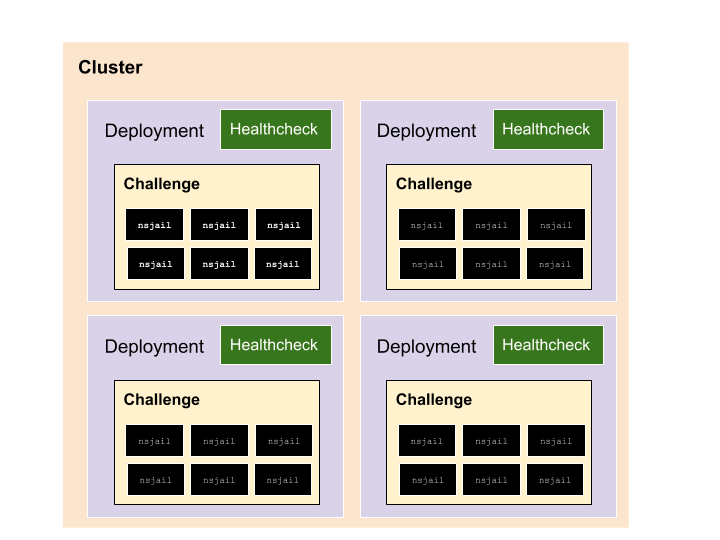
\includegraphics[width=0.85\linewidth,height=0.65\textheight,keepaspectratio]{src/images/kctf-architecture.png}
  \caption{Kctf Architecture}
  \label{fig:kctf-architecture}
\end{figure}


Facendo riferimento all\textquotesingle immagine sopra,
l\textquotesingle architettura di kCTF prevede:

\begin{itemize}
\tightlist
\item
  Un \textbf{cluster}, che contiene un\textquotesingle insieme di
  challenge
\item
  Dei \textbf{deployment}, ognuno contiene due container (o meglio, un
  Pod che instanzia 2 container):

  \begin{itemize}
  \tightlist
  \item
    un container \passthrough{\lstinline!healthcheck!}: usato per
    determinare lo stato di salute dei servizi
  \item
    un container \passthrough{\lstinline!challenge!}: contiene i servizi
    su cui lavora lo sfidante.
  \end{itemize}
\end{itemize}

\begin{quote}
\textbf{Pod}: in Kubernetes, e\textquotesingle{} la piu piccola unita
che Kubernetes puo\textquotesingle{} eseguire. Un Pod, rappresenta uno o
piu container in esecuzione su un singolo nodo.\footnote{\label{fn:ref_7}\url{https://www.k8s.guide/workloads/pods-deployments/}}
\end{quote}

\begin{quote}
\textbf{Deployment}: in Kubernetes, un deployment e\textquotesingle{} un
template che specifica come creare i container. I template guidano la
creazione di \textbf{Pods} e la gestione sicura del ciclo di vita di un
Pod, in particolare la gestione dei ReplicaSet.\footref{fn:ref_7}
\end{quote}

NSJail viene avviato su ogni container
\passthrough{\lstinline!challenge!}, ed e\textquotesingle{} configurato
per ascoltare su una porta TCP nota. Ad ogni connessione TCP in arrivo,
NSJail esegue un fork restituendo allo sfidante
un\textquotesingle ambiente separato (rispetto agli altri sfidanti) su
cui lavorare. L\textquotesingle obiettivo di questa architettura
e\textquotesingle{} di poter riutilizzare lo stesso container per piu
sfidanti.

L\textquotesingle isolamento fornito da NSJail, si ottiene combinando
varie tecniche:

\begin{itemize}
\tightlist
\item
  Creazione di nuovi namespace: l\textquotesingle ambiente fornito,
  esegue su un nuovo namespace, separando logicamente le risorse
  accessibili.
\item
  Filtraggio delle chiamate di sistema tramite
  \passthrough{\lstinline!seccomp-bpf!}: questo sottosistema permette di
  uccidere i processi nell\textquotesingle ambiente se vengono eseguite
  chiamate di sistema vietate.
\item
  Accounting e limitazione delle risorse con
  \passthrough{\lstinline!cgroup!}: questo sottosistema permette di
  monitorare e limitare le risorse utilizzabili nel nuovo ambiente.
\end{itemize}

NsJail puo\textquotesingle{} essere configurato in modo che ogni
ambiente isolato, abbia a disposizione un\textquotesingle filesystem
temporaneo che risiede in RAM, mentre il filesystem originale
e\textquotesingle{} accessibile dall\textquotesingle ambiente sandbox in
sola lettura. Questa configurazione e\textquotesingle{} necessaria
poiche altrimenti gli sfidanti modificherebbero tutti lo stesso
filesystem.

Un\textquotesingle altra configurazione di NSJail e\textquotesingle{} la
seguente: che e\textquotesingle{} ideale per le challenge di tipo
\passthrough{\lstinline!pwn!} (trovare e sfruttare vulnerabilita in file
binari):

\begin{lstlisting}
[...]
mount: [
  {
    src: "/chroot"
    dst: "/"
    is_bind: true
  },
  {
    dst: "/tmp"
    fstype: "tmpfs"
    rw: true
  },
  {
    dst: "/proc"
    fstype: "proc"
    rw: true
  },
  {
    src: "/etc/resolv.conf"
    dst: "/etc/resolv.conf"
    is_bind: true
  }
]
\end{lstlisting}

\begin{enumerate}
\def\labelenumi{\arabic{enumi}.}
\tightlist
\item
  La cartella \passthrough{\lstinline!/chroot!} che risiede nel
  container, diventa la radice nel nuovo ambiente.
\item
  Viene creato un nuovo \passthrough{\lstinline!tmpfs!}, in
  \passthrough{\lstinline!/tmp!}
\item
  Viene importata la configurazione DNS da
  \passthrough{\lstinline!/etc/resolv.conf!} dentro la nuova radice.
\end{enumerate}

Tutta via, l\textquotesingle uso di NsJail per separare gli ambienti dei
partecipanti, rende difficoltosa l\textquotesingle implementazione di
challenge in cui si vuole dare la liberta ai partecipanti di installare
pacchetti dentro al container, oppure di modificare file di
configurazione che risiedono per esempio in
\passthrough{\lstinline!/etc!} e di modificare direttamente servizi in
esecuzione sul container. \footnote{\label{fn:ref_8}\url{https://github.com/google/kctf/blob/v1/docs/security-threat-model.md}}

Queste limitazioni ci sono perche NsJail nell\textquotesingle ambiente
sandbox non fornisce una propria istanza di
\passthrough{\lstinline!systemd!} (o un qualsiasi gestore di servizi) e
neanche l\textquotesingle infrastruttura necessaria per eseguiure
comandi come \passthrough{\lstinline!apt!}.

Tale limitazione, porta ad escludere kCTF come possibile soluzione al
problema orignale esposto, suggerendo come astrazione migliore per
l\textquotesingle ambiente di un partecipante l\textquotesingle uso di
un \textbf{container} (Incus o Docker), piuttosto che una sandbox
generata da NsJail.

TODO: \textbf{Problemi}:

\begin{itemize}
\tightlist
\item
  in nsjail il filesystem e\textquotesingle{} disponibile in sola
  lettura. Comandi come \passthrough{\lstinline!apt!} e modifiche
  diretta a \passthrough{\lstinline!/etc!} non funzionano.
\item
  se la connessione TCP cade allora tutto il lavoro che risiede in RAM
  e\textquotesingle{} perso
\item
  in nsjail, l\textquotesingle applicazione di filtri seccomp potrebbero
  impedire l\textquotesingle esecuzione di alcune chiamate di sistema.
\item
  kCFT usa Kubernetes introducendo costi e complessita.
\end{itemize}

\subsection{CR Alternativi: CTFBox}\label{cr-alternativi-ctfbox}

CTFBox e\textquotesingle{} un Cyber Range perfetto per organizzare CTF
di tipo Attack/Defense, dove ogni team ha una macchina con uno o piu
servizi vulnerabili da difendere, mentre si attaccano i servizi esposti
sulle macchine avversarie per recuperare le flag. Durante il gioco, ogni
team deve fare attenzione a non rompere i propri servizi, mantenendo
un\textquotesingle alta percentuale di SLA. Una SLA bassa comporta una
penalita\textquotesingle{} in termini di punteggio. \footnote{\label{fn:ref_9}\url{https://ctfbox.domy.sh/}}

Fa uso di \textbf{Docker} per gestire i servizi essenziali del gioco (e
che costituiscono quindi CTFBox), mentre \textbf{Incus} viene utilizzato
per gestire l\textquotesingle esecuzione delle macchine virtuali o dei
container dei team.


\begin{figure}[htbp]
  \centering
  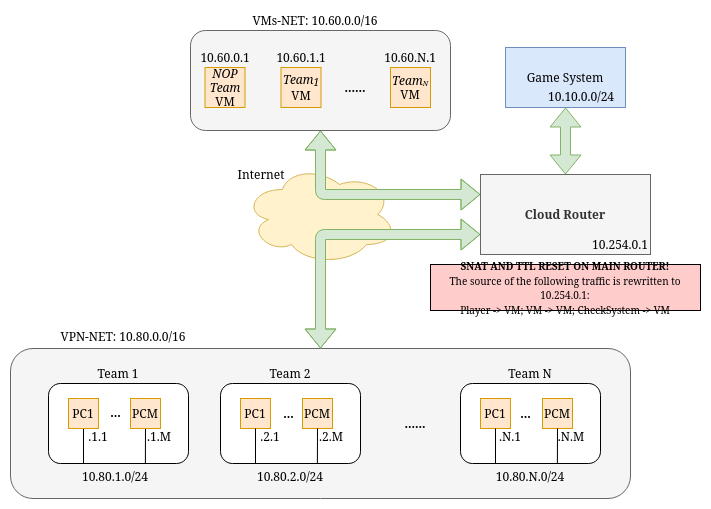
\includegraphics[width=0.85\linewidth,height=0.65\textheight,keepaspectratio]{src/images/ctfbox-architecture.png}
  \caption{Ctfbox Architecture}
  \label{fig:ctfbox-architecture}
\end{figure}


\textbf{Router}: e\textquotesingle{} un container Docker, che gestisce
le configurazioni della rete WireGuard, permettendo ai giocatori di
connettersi alla rete di gioco. Controlla le regole di routing sulla
rete, e governa la transizione della rete tra 3 stati diversi:

\begin{itemize}
\tightlist
\item
  \passthrough{\lstinline!freeze!}: in questo stato, nessuno
  puo\textquotesingle{} accedere alle macchine vulnerabili
\item
  \passthrough{\lstinline!lock!}: in questo stato, ogni team
  puo\textquotesingle{} accedere solo alla propria macchina vulnerabile.
\item
  \passthrough{\lstinline!unlock!}: in questo stato, la rete
  e\textquotesingle{} completamente aperta, i team possono attaccare le
  macchine avversarie.
\end{itemize}

\textbf{Game System}: e\textquotesingle{} un container Docker, che
agisce da cervello centrale per la gestione del gioco.

\begin{itemize}
\tightlist
\item
  Gestisce lo stato della rete (freeze/lock/unlock), comunicando i
  cambiamenti al router.
\item
  Mantiene il database delle flag, e calcola i punteggi per ogni team.
\item
  Coordina i Checkers, ossia i worker che interrogano i servizi dei team
  ad ogni tick.
\end{itemize}

In CTFBox, ad ogni tick (ossia ogni round di gioco), le flag vengono
rigenerate su ogni macchina, per ogni servizio vulnerabile, e registrate
nel database. L\textquotesingle obiettivo di un team in una competizione
Attack/Defense strutturata in questo modo e\textquotesingle{} di
attaccare piu volte lo stesso servizio sulle macchine avversarie, per
recuperare quante piu flag possibli, finche le difese avversarie non
bloccano gli attacchi.

\textbf{Checkers}, ad ogni tick (o round) fanno due cose:

\begin{enumerate}
\def\labelenumi{\arabic{enumi}.}
\tightlist
\item
  Interrogano tutti i servizi vulnerabili attivi, e determinano la
  percentuale di SLA per ogni team.
\item
  Installano le nuove flag sui servizi vulnerabili.
\end{enumerate}

Ogni membro del team, ha la sua configurazione \textbf{WireGuard} per
conettersi alla propria macchina e per raggiungere le macchine
avversarie. Ad ogni giocatore che si connette viene assegnato
un\textquotesingle indirizzo nella sottorete
\passthrough{\lstinline!10.80.team\_id.0/24!} mentre le macchine dei
team si trovano nella sottorete \passthrough{\lstinline!10.60.0.0/16!}.

Dunque CTFBox si rileva essere un\textquotesingle ottimo sistema per
gestire competizioni Attack/Defense e per regolare
l\textquotesingle accesso alle macchine, ma la sua architettura non si
applica in contesti in cui vorremmo solo assegnare ad ogni team un
insieme di macchine vulnerabili il cui stato verra\textquotesingle{} poi
verificato da un\textquotesingle oracolo.

\subsection{CR Alternativi: CyTrONE}\label{cr-alternativi-cytrone}

\textbf{CyTrONE}\footnote{\label{fn:ref_10}\url{https://github.com/crond-jaist/cytrone}}
e\textquotesingle{} un framework incentrato sul training che integra
contemporaneamente sia una piattaforma educativa che un Cyber Range.

La seguente immagine mostra i componenti di CyTrONE:

\begin{figure}[htbp]
  \centering
  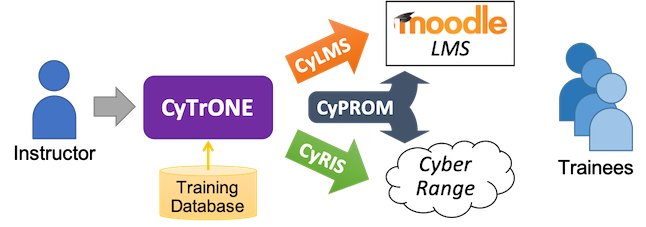
\includegraphics[width=0.85\linewidth,height=0.65\textheight,keepaspectratio]{src/images/cytrone-architecture.png}
  \caption{Cytrone Architecture}
  \label{fig:cytrone-architecture}
\end{figure}


\begin{itemize}
\tightlist
\item
  \textbf{CyLMS}: si occupa d icaricare il contenuto per il training su
  un Learning Management System come \textbf{Moodle}
\item
  \textbf{CyRIS} (Cyber Range Instantiation System): si occupa di
  istanziare l\textquotesingle ambiente di training su cui gli studenti
  possono condurre opportuni test per avanzare nel training.
\item
  \textbf{CyPROM}: si occupa di tracciare l\textquotesingle avanzamento
  controllando LMS ed il Cyber Range.
\end{itemize}

CyTrONE gestisce tre tipi di training\footnote{\label{fn:ref_11}\url{https://www.sciencedirect.com/science/article/pii/S0167404818306527}}:

\begin{itemize}
\tightlist
\item
  Training \emph{Attack-oriented}: si basa sul capire come riprodurre
  attacchi a vulnerabilita note.
\item
  Training \emph{Analysis-oriented}: si concentra
  sull\textquotesingle analisi dell\textquotesingle attacco, per capire
  come funziona e le sue conseguenze.
\item
  Training \textbf{Defense-oriented}: si conentra sulle tecniche di
  patching delle vulnerabilita, al fine di proteggere il sistema.
\end{itemize}

Quindi l\textquotesingle esperienza utente si concentra sul fatto che
gli studenti possono eseguire un training e visualizzare le risorse
associate sul Moodle ed al tempo stesso accedere al Cyber Range
associato.

CyTrONE si applica bene facendo le seguenti assunzioni:

\begin{quote}
\begin{enumerate}
\def\labelenumi{\arabic{enumi})}
\tightlist
\item
  \emph{L\textquotesingle obiettivo di ciascuna attività di formazione
  può essere formulato come un problema, che può dipendere o meno da
  altri problemi della stessa lezione (es: trova
  l\textquotesingle indirizzo IP, trova la flag);} \footref{fn:ref_11}
\end{enumerate}
\end{quote}

\begin{quote}
\begin{enumerate}
\def\labelenumi{\arabic{enumi})}
\setcounter{enumi}{1}
\tightlist
\item
  \emph{Il sistema è in grado di stabilire automaticamente se il
  partecipante abbia risolto il problema, confrontando la risposta
  fornita con un valore noto} \footref{fn:ref_11}
\end{enumerate}
\end{quote}

L\textquotesingle architettura di CyTrONE e\textquotesingle{} supportata
da un \emph{Training Database}, che si occupa di tenere in memoria le
informazioni per i vari training, che vengono caricate su CyTrONE da una
figura identificata come \emph{Training Coordinator}.Le informazioni
mantenute nel database sono per esempio: il training content, file e
programmi, macchine virtuali, ecc... \footref{fn:ref_11}

CyTrONE utilizza un file YAML per definire il contenuto di un training:

\begin{figure}[htbp]
  \centering
  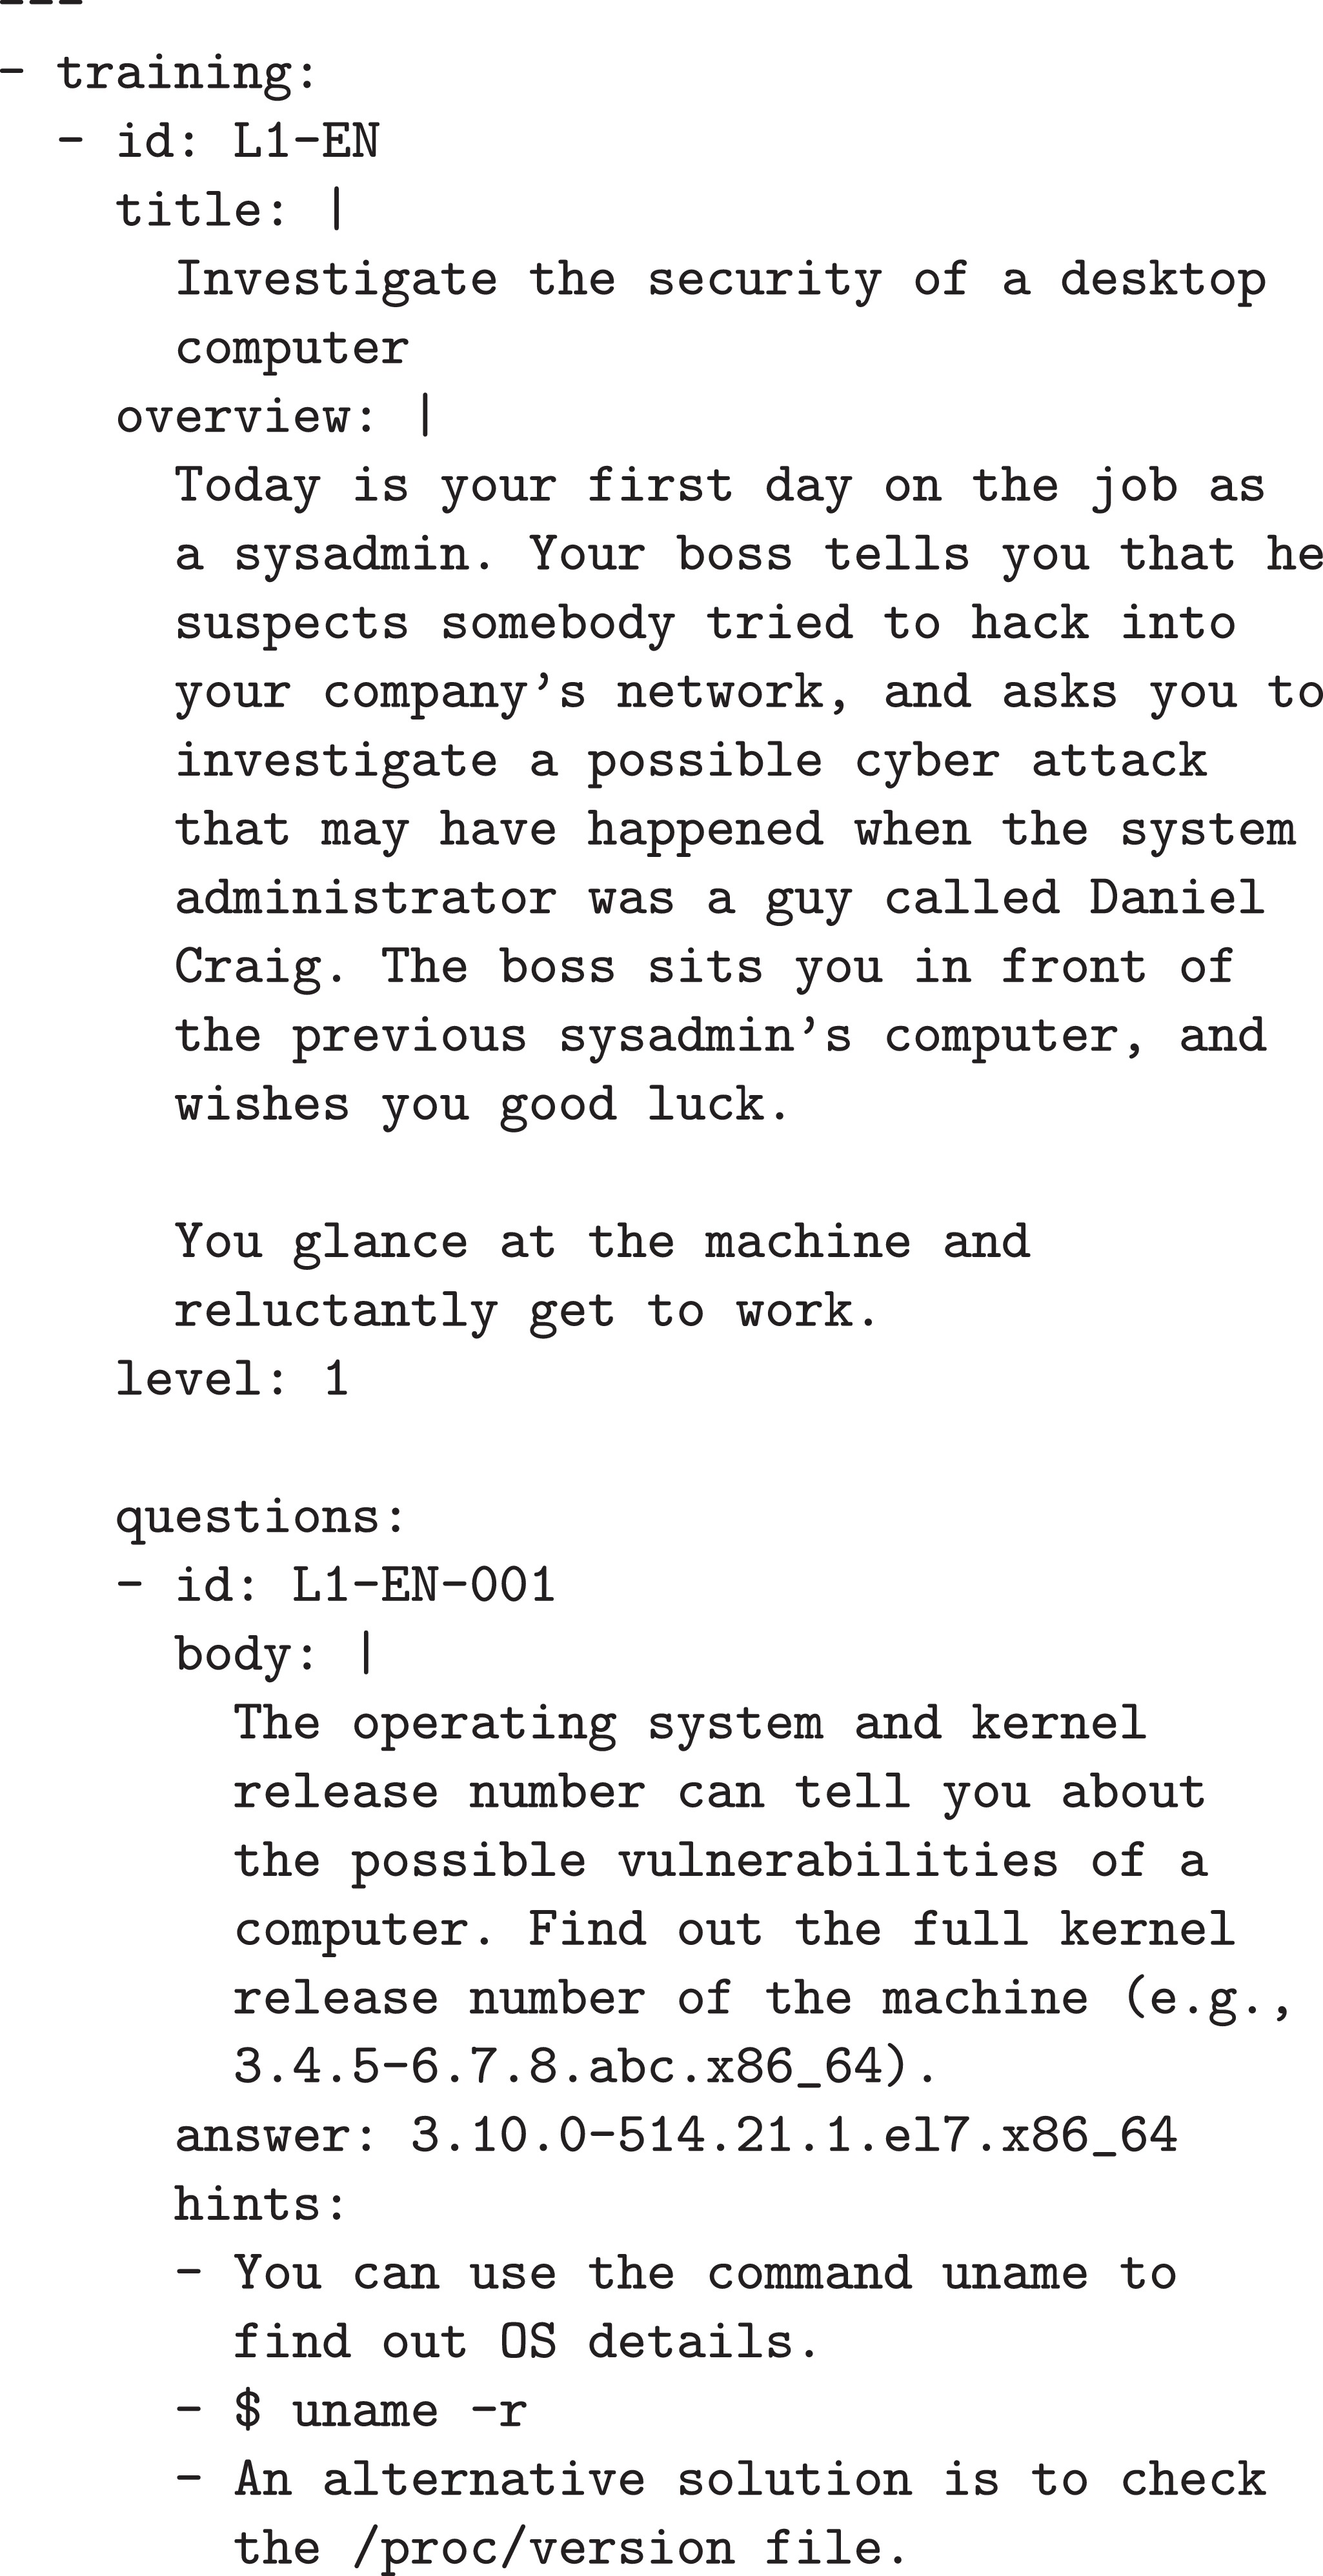
\includegraphics[width=0.85\linewidth,height=0.65\textheight,keepaspectratio]{src/images/cytrone-training.png}
  \caption{Cytrone Training}
  \label{fig:cytrone-training}
\end{figure}


E similmente, si usa un file YAML per definire la specifica del Cyber
Range: 
\begin{figure}[htbp]
  \centering
  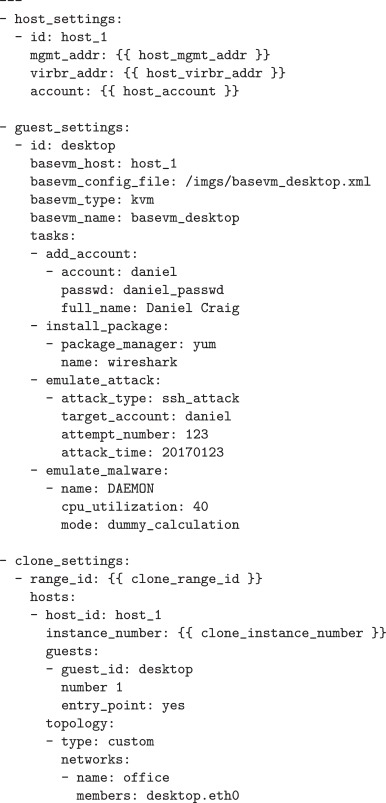
\includegraphics[width=0.85\linewidth,height=0.65\textheight,keepaspectratio]{src/images/cytrone-cyberrange.png}
  \caption{Cytrone Cyberrange}
  \label{fig:cytrone-cyberrange}
\end{figure}


A partire dalla configurazione YAML del Cyber Range, il sotto-sistema
CyRIS si occupa di istanziarlo. Successivamente, in caso di un training
\textbf{Defense-oriented} l\textquotesingle utente richiede
l\textquotesingle attacco associato alla vulnearbilita
all\textquotesingle interno del sistema e ne viene registrato
l\textquotesingle esisto.

Tutta via, sebbene il sistema sia ben ingegnerizzato soffre di alcuni
problemi:

\begin{enumerate}
\def\labelenumi{\arabic{enumi}.}
\tightlist
\item
  Il deploy delle vulnerabilita avviene su macchine virtuali, che
  possono costituire un alto overhead in termini di risorse, ed tempi di
  approvvigionamento lunghi per l\textquotesingle infrastruttura.
\item
  Il payload viene inviato remotamente dal
  \passthrough{\lstinline!cyberattack controller!} (che non fa altro che
  eseguire \passthrough{\lstinline!Metasploit!}). Tutta via il traffico
  di rete puo\textquotesingle{} essere intercettato dallo studente,
  ottenendo cosi suggerimenti per la soluzione.
\item
  L\textquotesingle esecuzione del payload puo scatenare la produzione
  di file log accessibili allo studente.
\item
  Necessita di un LMS (per design) per tenere traccia del training
  progress.
\end{enumerate}

TODO: analisi del grafico!

% Sezione vuota






\fancyhead[R]{\rightmark} \fancyhead[L]{\leftmark}
\fancyfoot[R]{\thepage}\fancyfoot[L]{\leftmark}


% ELENCO DELLE FIGURE (OPZIONALE)
\addcontentsline{toc}{chapter}{Elenco delle figure}
\listoffigures
\addcontentsline{toc}{chapter}{Elenco dei codici}
\lstlistoflistings
\addcontentsline{toc}{chapter}{Elenco degli algoritmi}
\listofalgorithms


% BIBLIOGRAFIA
\bibliographystyle{IEEEtran} 
\bibliography{Bibliography}


\end{document}